\section{Content}
\label{section:content}

\subsection{DDoS Attacks and BRO}\label{subsec:ddos-and-bro}
In this section we will first define the notion of a DDoS attack by explaining how the infrastructure looks like. Then we will elaborate on various DDoS attacks used nowadays and discuss their main characteristics. After this we will discuss the syntax of the detection rules of the BRO SIDS.

\subsubsection{The DDoS Attack}
Figure \ref{fig:ddos-overview} shows the infrastructure of a DDoS attack. Actors involved in a DDoS attack are denoted by a letter (A-D) whereas data streams are denoted by numbers (1-5). 

A DDoS attack starts with an attacker (A). The attacker sends data needed to start the attack (1) to the Command and Control (C\&C) servers (B). The C\&C servers control the infected machines (C). The infected machines are also known under the name of bots. The C\&C servers plus the infected machines are more commonly named as a botnet. The C\&C servers send a message (2) to the infected machines. In case of the Ramnit botnet, only the infected machines counted 3.2 million machines \cite{europol2015}. At this point two paths are used to get to the target machine (E). The first path possible is aiming the infected machines directly to the target (4). The second path possible is using public services (D) like a DNS to reach the target (5). 

In the next subsection we will describe various types of DDoS attacks. 

\begin{figure}[H]
\centering
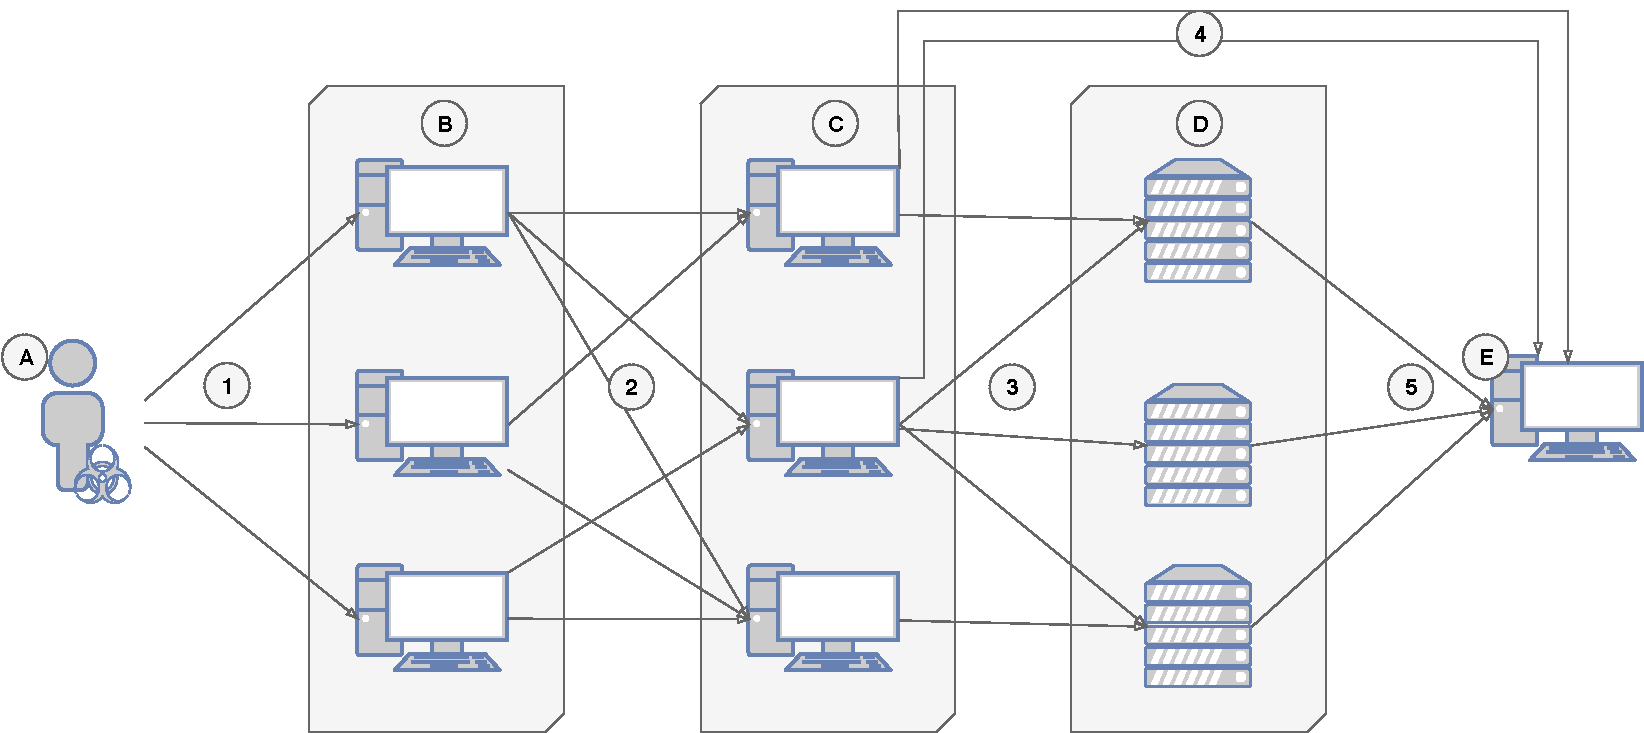
\includegraphics[width=\textwidth]{./images/ddos-overview.pdf}
\caption{Overview of DDoS attack infrastructure}
\end{figure}\label{fig:ddos-overview}

\subsubsection{Types of Attacks}
In this section we will briefly elaborate on various types of attack. The main characteristics can be found in Table $\dots$.

\paragraph{UDP Fragment}



\subsubsection{BRO Rule Syntax} 


\subsection{Methodology}\label{subsec:methodology}

\subsection{Evaluation and Discussion}\label{subsec:evaluation-discussion}
\subsubsection{Evaluation}\label{subsubsec:evalutation}
\subsubsection{Discussion}\label{subsubsec:discussion}
